\documentclass[compress]{beamer}
\usepackage{ifthen,verbatim,ulem}

\newcommand{\isnote}{}
\xdefinecolor{lightyellow}{rgb}{1.,1.,0.25}
\xdefinecolor{darkblue}{rgb}{0.1,0.1,0.7}
\xdefinecolor{darkgreen}{rgb}{0.1,0.7,0.1}

%% Uncomment this to get annotations
%% \def\notes{\addtocounter{page}{-1}
%%            \renewcommand{\isnote}{*}
%% 	   \beamertemplateshadingbackground{lightyellow}{white}
%%            \begin{frame}
%%            \frametitle{Notes for the previous page (page \insertpagenumber)}
%%            \itemize}
%% \def\endnotes{\enditemize
%% 	      \end{frame}
%%               \beamertemplateshadingbackground{white}{white}
%%               \renewcommand{\isnote}{}}

%% Uncomment this to not get annotations
\def\notes{\comment}
\def\endnotes{\endcomment}

\setbeamertemplate{navigation symbols}{}
\setbeamertemplate{headline}{\mbox{ } \hfill
\begin{minipage}{5.5 cm}
\vspace{-0.75 cm} \small
\end{minipage} \hfill
\begin{minipage}{4.5 cm}
\vspace{-0.75 cm} \small
\begin{flushright}
\ifthenelse{\equal{\insertpagenumber}{1}}{}{Jim Pivarski \hspace{0.2 cm} \insertpagenumber\isnote/\pageref{numpages}}
\end{flushright}
\end{minipage}\mbox{\hspace{0.2 cm}}\includegraphics[height=1 cm]{../cmslogo} \hspace{0.1 cm} \includegraphics[height=1 cm]{../tamulogo} \hspace{0.01 cm} \vspace{-1.05 cm}}

\begin{document}
\begin{frame}
\vfill
\begin{center}
\textcolor{darkblue}{\Large Muon Alignment Constants Proposed for Sign-off \\ \vspace{0.2 cm}(for CRAFT and Cosmic Ray Monte Carlo)}

\vfill
\begin{columns}
\column{0.3\linewidth}
\begin{center}
\large
\textcolor{darkblue}{Jim Pivarski}
\end{center}
\end{columns}

\begin{columns}
\column{0.3\linewidth}
\begin{center}
\scriptsize
{\it Texas A\&M University}
\end{center}
\end{columns}

\vspace{0.5 cm}
for the Muon Alignment Community

\vfill
 3 June, 2009

\end{center}
\end{frame}

%% \begin{notes}
%% \item This is the annotated version of my talk.
%% \item If you want the version that I am presenting, download the one
%% labeled ``slides'' on Indico (or just ignore these yellow pages).
%% \item The annotated version is provided for extra detail and a written
%% record of comments that I intend to make orally.
%% \item Yellow notes refer to the content on the {\it previous} page.
%% \item All other slides are identical for the two versions.
%% \end{notes}

\small

\begin{frame}
\frametitle{New sets of constants}
\begin{itemize}\setlength{\itemsep}{0.4 cm}
\item DTAlignmentRcd for CRAFT
\begin{itemize}\setlength{\itemsep}{0.1 cm}
\item internal DT alignment from tracks, independently confirmed by survey
\item global DT positions and angles from tracks, tested with
  relative differences and high-$p_T$ momentum reconstruction
\end{itemize}

\item CSCAlignmentRcd for CRAFT
\begin{itemize}\setlength{\itemsep}{0.1 cm}
\item individual chambers relative to disks from photogrammetry
\item disk-bending due to $\vec{B}$ from laser measurements
\item whole-disk positions relative to tracker from tracks
\end{itemize}

\item Updated STARTUP Scenario for Monte Carlo
\begin{itemize}\setlength{\itemsep}{0.1 cm}
\item includes the above improvements
\item only appropriate for pre-collisions MC
\end{itemize}
\end{itemize}
\end{frame}

\begin{frame}
\frametitle{Internal DT alignment}

\begin{columns}
\column{0.35\linewidth}
\begin{itemize}\setlength{\itemsep}{0.25 cm}
\item \mbox{Physically-motivated corrections\hspace{-3 cm}} \\ \mbox{to internal chamber geometry\hspace{-3 cm}} \\ \mbox{(superlayers): layer of glue,\hspace{-3 cm}} \\ \mbox{about 1~mm thick in $z$\hspace{-3 cm}}

\item \mbox{Track-based measurement\hspace{-3 cm}} \\ \mbox{($x$ residuals versus\hspace{-3 cm}} \\ \mbox{entrance angle) and\hspace{-3 cm}} \\ survey agree in $z$

\item 540~$\mu$m verification in station~1 (plot)

\item Track-based $x$ corrections also improve whole-chamber segment angles
\end{itemize}

\column{0.65\linewidth}
\hfill 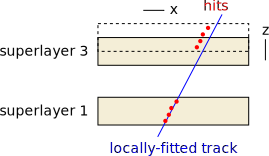
\includegraphics[width=0.7\linewidth]{internal_dt.pdf}

\vspace{0.5 cm}
\includegraphics[width=\linewidth]{internal_alignment.png}
\end{columns}
\end{frame}

\begin{frame}
\frametitle{Global DT alignment}
\begin{itemize}
\item Align individual muon chambers relative to tracker with tracker-only refits of globalMuons (unbiased residuals)
\item Fully 6-DOF procedure, fitting for all alignment corrections and major instrumental/propagation effects together, once per chamber
\begin{itemize}
\item four residuals: $x$, $y$ position and $\frac{dx}{dz}$, $\frac{dy}{dz}$ entrance angle
\item correlation between position and angle residuals included
\item single-scattering (power-law) convoluted with Gaussian errors
\end{itemize}
\item $100 < p_T < 200$~GeV, because low-$p_T$ tracks are biased by an effect {\it other than} magnetic field map or material budget errors
\item Consistent with tracker geometry in Tracker\_Geometry\_v5\_offline
\item Region aligned: wheels $-$1, 0, $+$1, all sectors except 1 and 7
\item Realistic cosmic ray Monte Carlo study \mbox{(except tracker misalignment);\hspace{-1 cm}} \\ achieved the following systematics-dominated accuracy:
\begin{center}
\begin{tabular}{c c c c}
$x$ & 190~$\mu$m & $\phi_x$ & 0.42~mrad \\
$y$ & 840~$\mu$m & $\phi_y$ & 0.09~mrad \\
$z$ & 630~$\mu$m & $\phi_z$ & 0.29~mrad
\end{tabular}
\end{center}
\item Up-to-date alignment code in CVS (and 3\_1\_0 release)
\end{itemize}
\end{frame}

\begin{frame}
\frametitle{Example in real data}
\begin{itemize}
\item Wheel~0, station~1, sector~10 (largest statistics, bottom of CMS)
\end{itemize}

\vfill
\mbox{\hspace{-0.85 cm}\begin{minipage}{1.1\linewidth}
\begin{tabular}{p{0.5\linewidth} p{0.5\linewidth}}
\mbox{ } \hfill \textcolor{darkblue}{\normalsize Before (misaligned)} \hfill \mbox{ } & \mbox{ } \hfill \textcolor{darkblue}{\normalsize After (aligned)} \hfill \mbox{ } \\
\includegraphics[height=\linewidth, angle=90]{exampleData_wh0st1sec10_bellbefore.pdf} & \includegraphics[height=\linewidth, angle=90]{exampleData_wh0st1sec10_bellafter.pdf} \\
\includegraphics[height=\linewidth, angle=90]{exampleData_wh0st1sec10_polybefore.pdf} & \includegraphics[height=\linewidth, angle=90]{exampleData_wh0st1sec10_polyafter.pdf} \\
\end{tabular}\end{minipage}}
\end{frame}

\begin{frame}
\frametitle{Parameter updates}
\begin{itemize}
\item Differences between proposed constants and previous (CRAFT\_ALL\_V5--12) shown below
\item Systematic rotation of wheels is due to low-$p_T$ tracks used in previous alignment
\end{itemize}

\includegraphics[height=\linewidth, angle=90]{hip_difference_v11all.pdf}
\end{frame}

\begin{frame}
\frametitle{Momentum in split cosmics}
\begin{itemize}
\item $\frac{\left(1/p_T\right)_{\mbox{\tiny top}} - \left(1/p_T\right)_{\mbox{\tiny bot}}}{\sqrt{2} \, \left(1/p_T\right)_{\mbox{\tiny bot}}}$ (equal to $\frac{\left(p_T\right)_{\mbox{\tiny top}} - \left(p_T\right)_{\mbox{\tiny bot}}}{\sqrt{2} \, \left(p_T\right)_{\mbox{\tiny bot}}}$ if Gaussian)
\item $200 < p_T < 2000$~GeV tracks (not used in the alignment)
\item Key: \textcolor{red}{tracker-only,} sometimes with station~1, \textcolor{darkgreen}{with station~1,} \mbox{\textcolor{blue}{all stations}\hspace{-1 cm}}
\end{itemize}

\begin{minipage}{0.49\linewidth}\begin{center} \scriptsize CRAFT\_ALL\_V5--12 \end{center}\end{minipage}
\begin{minipage}{0.49\linewidth}\begin{center} \scriptsize new constants \end{center}\end{minipage}

\vspace{0.2 cm}
\includegraphics[width=0.5\linewidth]{R1n-pT2002000_7.png}
\includegraphics[width=0.5\linewidth]{R1n-pT2002000_4.png}

\hfill \textcolor{darkblue}{\scriptsize J.~Tucker}

\vspace{-\baselineskip}
\begin{minipage}{0.8\linewidth}
\begin{itemize}\setlength{\itemsep}{-0.05 cm}
\item \textcolor{red}{Tracker-only}: \hfill 4.51\%
\item Tracker and sometimes station~1: \hfill 5.33 $\to$ 4.36\%
\item \textcolor{darkgreen}{Tracker and muon station~1}: \hfill 6.76 $\to$ 4.50\%
\item \textcolor{blue}{Tracker and all muon stations}: \hfill 9.11 $\to$ 5.65\%
\end{itemize}
\end{minipage}
\end{frame}

\begin{frame}
\frametitle{DT alignment and 2008 MC}

\begin{itemize}\setlength{\itemsep}{0.35 cm}
\item 2008 MC $\frac{\left(1/p_T\right)_{\mbox{\tiny meas}} - \left(1/p_T\right)_{\mbox{\tiny gen}}}{\sqrt{2} \, \left(1/p_T\right)_{\mbox{\tiny gen}}}$ \textcolor{darkgreen}{tracker $+$ station~1} resolution:

\vspace{0.1 cm}
IDEAL: 2\%, CSA08 10~pb$^{-1}$: 3\%, STARTUP: 6\% at 200~GeV
\item Cosmic splitting $\frac{\left(1/p_T\right)_{\mbox{\tiny top}} - \left(1/p_T\right)_{\mbox{\tiny bot}}}{\sqrt{2} \, \left(1/p_T\right)_{\mbox{\tiny bot}}}$ \textcolor{darkgreen}{(same reco)}: 4.5\% at 200~GeV
\end{itemize}

\vspace{0.5 cm}
\hspace{-0.83 cm} \textcolor{darkblue}{\Large CSC alignment overview}

\begin{itemize}
\item Photogrammetry $+$ disk-bending (lasers) $+$ \mbox{disk positions (tracks)\hspace{-1 cm}}
\end{itemize}

\vspace{0.5 cm}
\hspace{-0.83 cm} \textcolor{darkblue}{\Large CSC photogrammetry}

\begin{itemize}
\item Describes individual chamber positions relative to their disks (300~$\mu$m resolution)
\item Not expected to move in $x$ and $y$ during 0~T $\to$ 3.8~T
\end{itemize}
\end{frame}

\begin{frame}
\frametitle{Disk-bending measurements}
\begin{itemize}
\item From Straight Line Monitor lasers and the Link System
\end{itemize}

\begin{center}\includegraphics[width=\linewidth]{hardware_alignment.png}\end{center}
\end{frame}

\begin{frame}
\frametitle{Disk positions}
\begin{itemize}
\item Local cathode strip residuals ($\approx r\phi$) as a function of chamber
\item Fit ME1/2 (2/2) to global $x$, $y$, $\phi_z$, cross-check with \mbox{ME1/3 (3/2)\hspace{-1 cm}}
\end{itemize}

\begin{columns}
\column{0.6\linewidth}
\includegraphics[height=\linewidth, angle=90]{endcap_mem22.pdf}

\includegraphics[height=\linewidth, angle=90]{endcap_mem32.pdf}

\column{0.4\linewidth}
\begin{itemize}\setlength{\itemsep}{0.25 cm}
\item Biggest correction: ME$-$2 and ME$-$3 

$\phi_z$: 1.44~mrad \\ $x$: 4.4~mm \\ $y$: $-$0.1~mm

\item ME$-$2/2 fit (top) is a good match to ME$-$3/2 (bottom)
\end{itemize}
\end{columns}
\end{frame}

\begin{frame}
\frametitle{Cross-checks for CSCs}

\begin{columns}
\column{0.65\linewidth}
\begin{itemize}
\item Raw globalMuon residuals (what we used for alignment): \mbox{improved by construction\hspace{-1 cm}}
\item $p_{\mbox{\scriptsize tracker}} - p_{\mbox{\scriptsize standAlone}}$ and standAlone $\chi^2$: no significant improvement (\textcolor{blue}{blue} is data)
\item We're continuing these studies, to align {\it individual} CSCs with tracks (difficult because of the angular distribution of cosmic rays)
\end{itemize}

\column{0.35\linewidth}
\includegraphics[width=\linewidth]{endcap_residuals.pdf}
\end{columns}

\vfill
\includegraphics[width=0.5\linewidth]{csc_p_comparison.png}
\includegraphics[width=0.5\linewidth]{csc_chi2_comparison.png}
\end{frame}

\begin{frame}
\frametitle{MC scenario}
\begin{itemize}
\item DT/CSC STARTUP misalignment scenario currently in the database
  describes the February CRAFT alignment (V5--12)
\item Since then\ldots
\begin{itemize}
\item more chambers have been aligned, with more degrees of freedom (within wheels $-$1, 0, $+$1)
\item resolution has improved due to updated algorithms
\item knowledge about resolution has improved: split cosmics
  techniques, $p_{\mbox{\scriptsize tracker}}/p_{\mbox{\scriptsize
      globalMuon}}$, relative position checks, Monte Carlo study
\end{itemize}
\item We've prepared a new geometry describing the state after CRAFT
\begin{itemize}
\item random-generator sigmas are explicitly derived from the cross-checks, alignment corrections, and MC study
\item unaligned chambers (wheels $\pm$2 and sectors 1 and 7) still have large misalignments
\end{itemize}
\item Appropriate for cosmic ray MC but not for physics: for \mbox{physics analyses,\hspace{-1 cm}} \\ we will align with collisions data (and therefore reach all chambers)
\end{itemize}
\end{frame}

%% \begin{frame}
%% \frametitle{Outline}
%% \begin{itemize}\setlength{\itemsep}{0.75 cm}
%% \item 
%% \end{itemize}
%% %% \hspace{-0.83 cm} \textcolor{darkblue}{\Large Outline2}
%% \end{frame}

%% \section*{First section}
%% \begin{frame}
%% \begin{center}
%% \Huge \textcolor{blue}{First section}
%% \end{center}
%% \end{frame}

\begin{frame}
\frametitle{Summary}
\begin{itemize}\setlength{\itemsep}{0.4 cm}
\item DTAlignmentRcd for CRAFT (2\_2\_X format)

{\tt \scriptsize /castor/cern.ch/user/p/pivarski/DTCRAFTiter03\_withCenteredTracker.db}

\item CSCAlignmentRcd for CRAFT (2\_2\_X format)

{\tt \scriptsize /castor/cern.ch/user/p/pivarski/CSCCRAFT\_HardwareAndPGAndDisk2.db}

\item Updated STARTUP Scenario for Monte Carlo

{\tt \scriptsize /castor/cern.ch/user/p/pivarski/MCScenario\_CRAFT1\_22X\_V02-09-04.db}

{\tt \scriptsize /castor/cern.ch/user/p/pivarski/MCScenario\_CRAFT1\_31X\_V02-09-04.db}

\end{itemize}
\label{numpages}
\end{frame}

\begin{frame}
\frametitle{Backup: relative DT positions}
\begin{columns}
\column{0.7\linewidth}
\begin{itemize}
\item Alignment determined positions of each chamber individually from the tracker
\item Cross-check with relative chamber positions
\item Measured from difference of residuals with respect to an unbiased track:

\mbox{(track $-$ station 3 hit) $-$ (track $-$ station 2 hit)}
\end{itemize}
\column{0.3\linewidth}
\includegraphics[width=\linewidth]{residuals_difference.pdf}
\end{columns}

\vspace{0.25 cm}
\begin{minipage}{0.24\linewidth}\begin{center} \scriptsize V5--12 $x$ \end{center}\end{minipage}
\begin{minipage}{0.24\linewidth}\begin{center} \scriptsize V5--12 $\phi_y$ \end{center}\end{minipage}
\begin{minipage}{0.24\linewidth}\begin{center} \scriptsize new $x$ \end{center}\end{minipage}
\begin{minipage}{0.24\linewidth}\begin{center} \scriptsize new $\phi_y$ \end{center}\end{minipage}

\includegraphics[width=0.25\linewidth]{diffxhist_v11.pdf} \includegraphics[width=0.25\linewidth]{diffphihist_v11.pdf} \includegraphics[width=0.25\linewidth]{diffxhist_may29.pdf} \includegraphics[width=0.25\linewidth]{diffphihist_may29.pdf}

\begin{itemize}
\item New $x$ resolution: 400~$\mu$m, with the exception of station~4, sector~4 chambers (which have internal structure, under investigation)
\item New $\phi_y$ resolution: 0.3--0.5~mrad
\end{itemize}
\end{frame}

\end{document}
